\section{Auswertung}
\label{sec:auswertung}
Im Folgenden werden alle Fehler mit Hilfe der \texttt{python}-Bibliothek
\texttt{uncertainties}\cite{py-uncertainties} berechnet, die eine Gaußsche
Fehlerfortpflanzung implementiert.

\subsection{Untersuchung an amplitudenmodulierten Schwingungen}
\label{subsec:am-auswertung}
Im Folgenden wird das Signal und Frequenzspektrum einer amplitudenmodulierten
Welle betrachtet. Anschließend wird das Signal mit Hilfe eines Ringmodulators,
sowie einer Gleichrichterdiode demoduliert.

\subsubsection{Amplitudenmodulation mit Ringmodulator}
\label{subsubsec:am-ringmodulator}
Das mit Hilfe eines Ringmodulators erzeugte Signal ist in Abbildung
\ref{fig:am-signal} dargestellt.
Das entsprechende Frequenzspektrum wird in Abbildung \ref{fig:am-spektrum}
gezeigt.
\begin{figure}
    \centering
    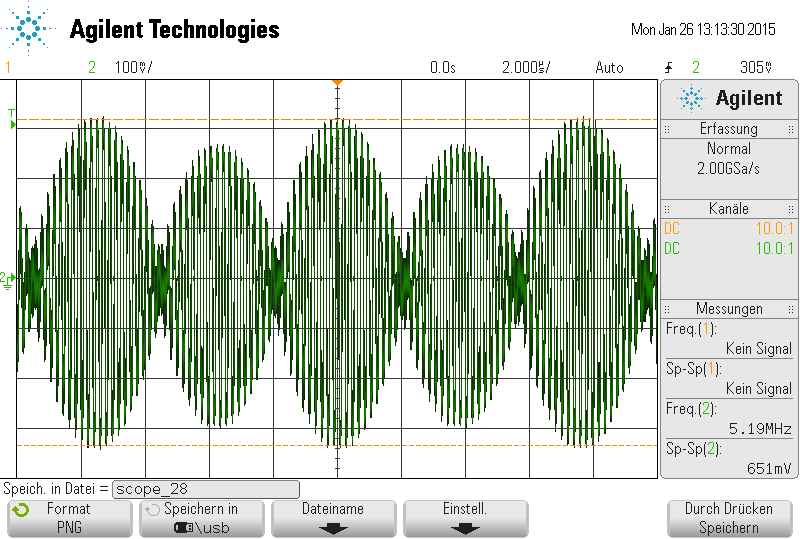
\includegraphics[width=0.8\linewidth]{images/am-signal.png}
    \caption{Amplitudenmoduliertes Signal.}
    \label{fig:am-signal}
\end{figure}
\begin{figure}
    \centering
    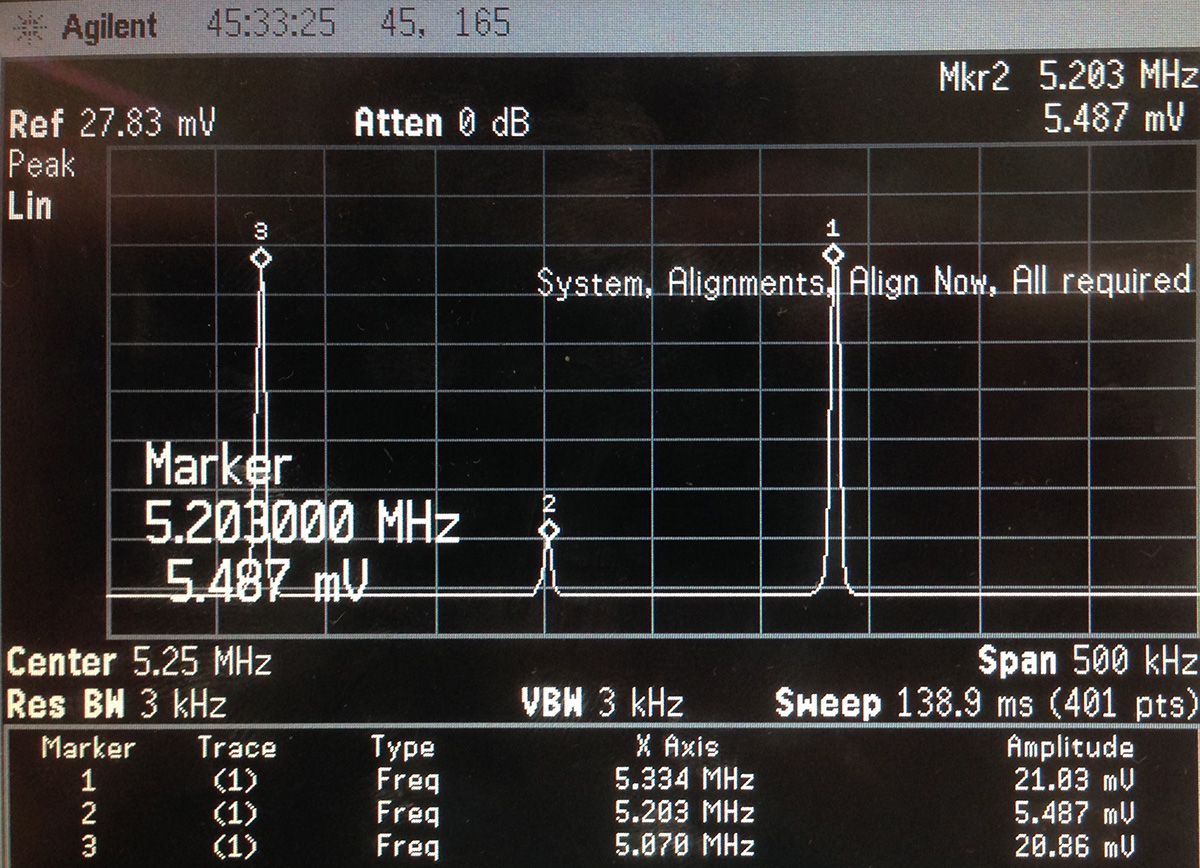
\includegraphics[width=0.8\linewidth]{images/am-spektrum.jpg}
    \caption{
        Frequenzspektrum des AM-Signals im Bereich um die
        Trägerfrequenz.
    }
    \label{fig:am-spektrum}
\end{figure}

\subsubsection{Amplitudenmodulation mit Diode}
\label{subsubsec:am-ringmodulator}
Die Amplitudenmodulation mit Hilfe einer Diode liefert das in Abbildung
\ref{fig:am-diode-signal}, beziehungsweise \ref{fig:am-diode-spektrum}
dargestellte Signal und Spektrum. Die Oberwellen der Trägerfrequenz bei
$2\omega_\text{T} = \SI{10.34}{\mega\hertz}$ und
$3\omega_\text{T} = \SI{15.53}{\mega\hertz}$ treten auf, weil XXX.
Sie sind in Abbildung \ref{fig:am-diode-oberwellen}

Der Modulationsgrad $m$ beträgt mit einer maximalen Schwebungsamplitude
von $U_\text{T}(1+m)=\SI{99.5}{\milli\volt}$ und einer minimalen Amplitude
von $U_\text{T}(1-m)=\SI{50.0}{\milli\volt}$
\begin{equation*}
    m_1 = \input{build/m1.tex}\,.
\end{equation*}
Mit Betrachtung des Frequenzspektrums ergibt sich bei einer Trägerfrequenz
$\omega_\text{T} = \SI{5.207}{\mega\hertz}$ und Seitenfrequenzen bei
$\omega_\text{T} + \omega_\text{M} = \SI{5.338}{\mega\hertz}$ und
$\omega_\text{T} - \omega_\text{M} = \SI{5.074}{\mega\hertz}$, sowie
entsprechenden Amplituden von $U_\text{T} = \SI{4.7+-0.1}{\milli\volt}$,
$U_1 = \SI{1.57+-0.01}{\milli\volt}$ und $U_2 = \SI{1.56+-0.01}{\milli\volt}$
der Modulationsgrad
\begin{equation*}
    m_2 = \input{build/m2.tex}\,.
\end{equation*}
\begin{figure}
    \centering
    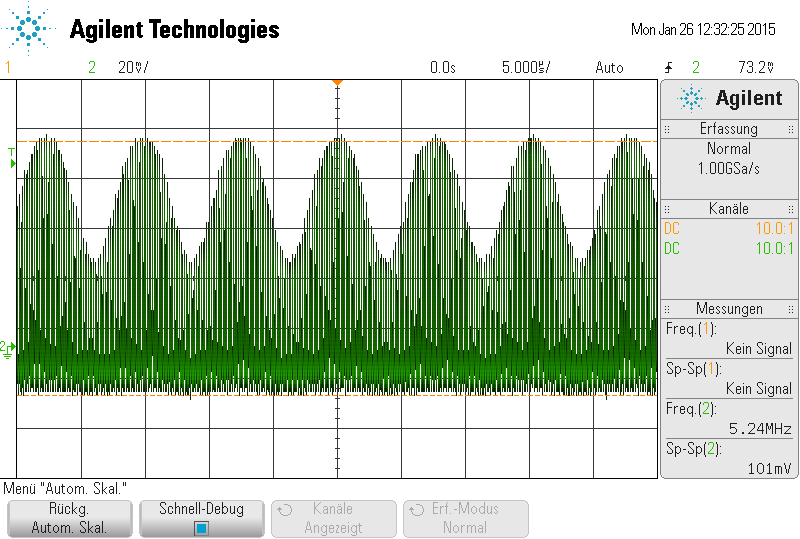
\includegraphics[width=0.8\linewidth]{images/am-diode-signal.png}
    \caption{Mit Hilfe einer Diode moduliertes Signal.}
    \label{fig:am-diode-signal}
\end{figure}
\begin{figure}
    \centering
    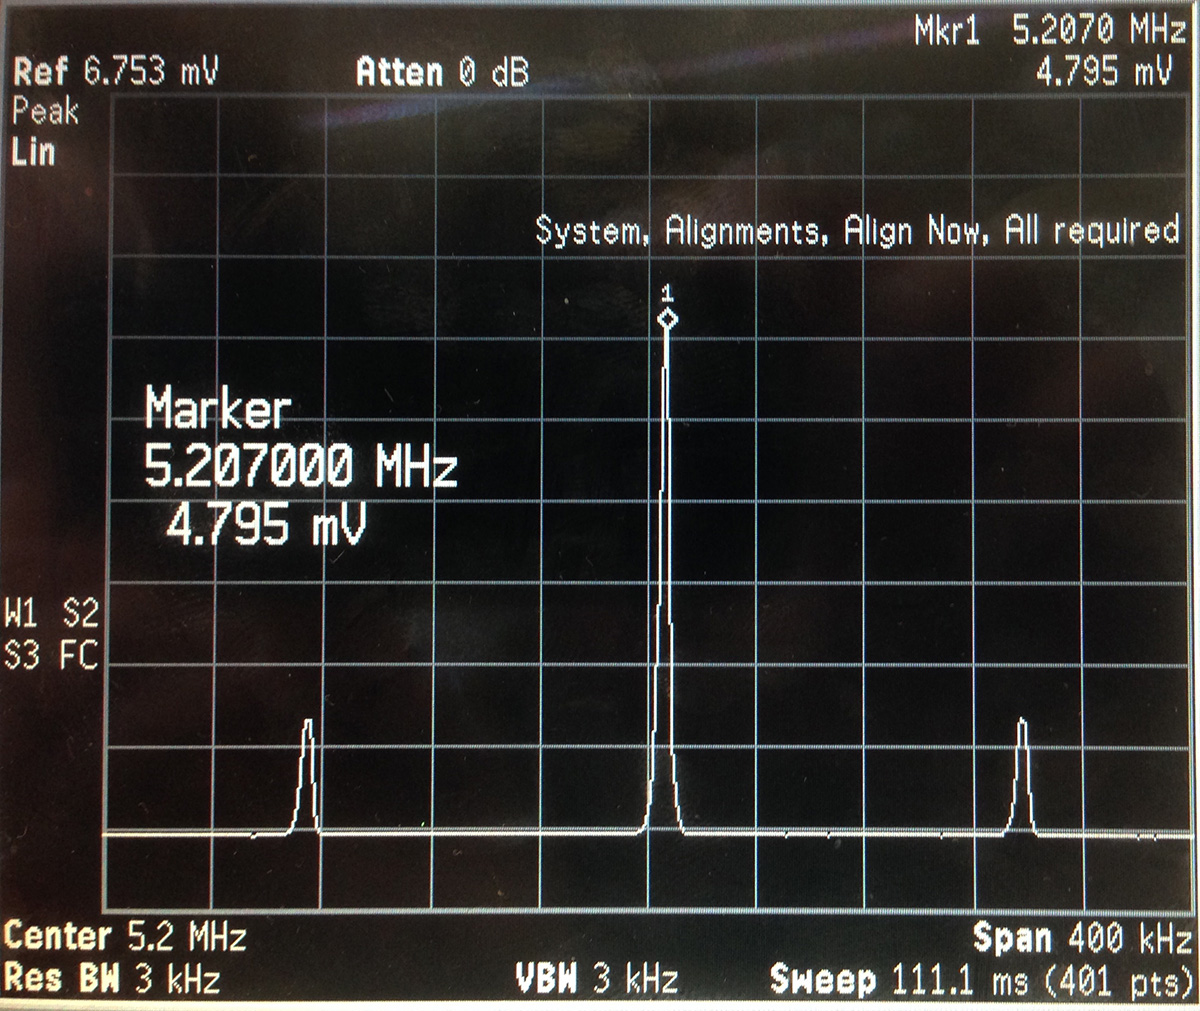
\includegraphics[width=0.8\linewidth]{images/am-diode-spektrum.jpg}
    \caption{
        Frequenzspektrum des mit Hilfe einer Diode erzeugten AM-Signals im
        Bereich um die Trägerfrequenz.
    }
    \label{fig:am-diode-spektrum}
\end{figure}
\begin{figure}
    \centering
    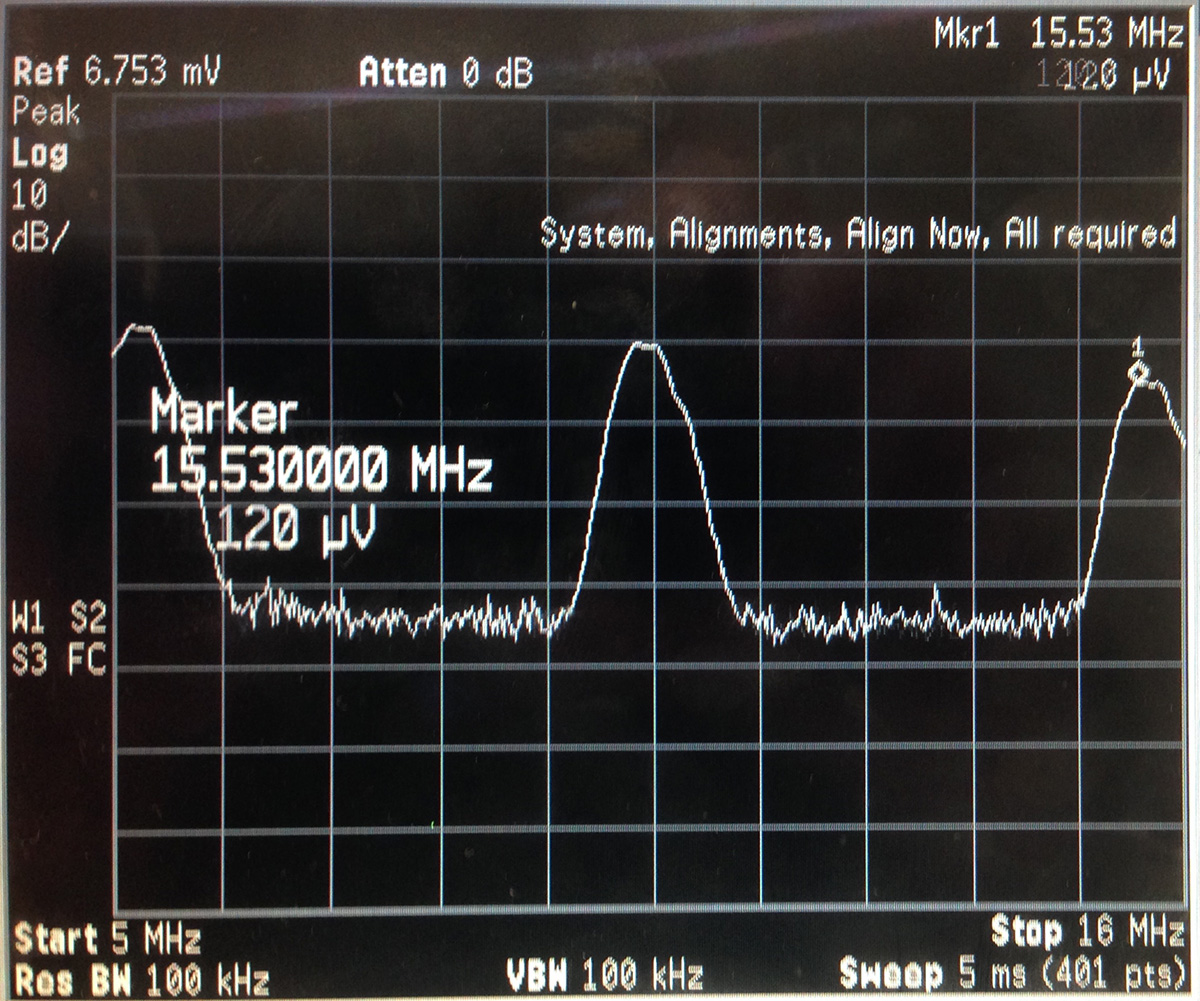
\includegraphics[width=0.8\linewidth]{images/am-diode-oberwellen.jpg}
    \caption{
        Oberwellen des AM-Singals.
    }
    \label{fig:am-diode-oberwellen}
\end{figure}

\subsubsection{Demodulation mit Ringmodulator}
\label{subsubsec:am-demodulation-ring}
Mit der in Abbildung XXX dargestellten Schaltung können AM-Signale mit
Kenntnis der Trägerspannung mit einem Ringmodulator demoduliert werden.
Zunächst wird die Abhängigkeit der Ausgangsspannung eines Ringmodulators
von der Phasendifferenz beider Eingangssignale untersucht. Dabei wird lediglich
eine Sinusspannung unterschiedlicher Laufzeit auf beide Eingänge gegeben.
Die Entsprechenden Messwerte sind in Tabelle \ref{tab:demodulation-cosinus}
aufgeführt und werden mitsamt einer Cosinus-Ausgleichsgerade in Abbildung
\ref{fig:demodulation-cosinus} dargestellt.
\begin{table}
    \centering
    \caption{Messwerte zur Bestimmung der Phasenabhängigkeit eines
    Ringmodulators}
    \label{tab:demodulation-cosinus}
    \begin{tabular}{SSSS}
        \toprule
        {$T/\si{\nano\second}$} & {$U/\si{\milli\volt}$} & {$T/\si{\nano\second}$} & {$U/\si{\milli\volt}$} \\
        \midrule
         0 &  76 & 24 & -125 \\ 
         4 &  42 & 28 & -151 \\ 
         8 &   8 & 32 & -155 \\ 
        12 & -23 & 36 & -136 \\ 
        16 & -58 & 40 & -103 \\ 
        20 & -91 & 44 &  -70 \\ 
        48 & -36 & 72 & 150 \\
        52 &  -4 & 76 & 151 \\
        56 &  13 & 80 & 128 \\
        60 &  61 & 84 &  96 \\
        64 &  95 & 88 &  62 \\
        68 & 127 & 92 &  30 \\
        \bottomrule
    \end{tabular}
\end{table}
\begin{figure}
    \centering
    \includegraphics[width=0.9\linewidth]{build/demodulation-cosinus.pdf}
    \caption{Phasenabhängigkeit eines Ringmodulators.}
    \label{fig:demodulation-cosinus}
\end{figure}
